\chapter{Parser}\label{chap:Parser}

In unserem \texttt{src/main/} Ordner wurde neben dem \texttt{Scanner/} Ordner der Ordner \texttt{Parser/} angelegt, der die wesentlichen Quellcode-Dateien enthält. In diesem Ordner befindet sich die \texttt{runParser.cpp}-Datei, welche die main-Methode enthält, die das eigentliche Programm startet. Hier werden die Programmparameter gelesen, also der Pfad für die Eingabe- und Ausgabedatei und die wesentlichen Objekte werden erstellt.

\section{Compiler}
Wenn man sich diese Funktion genauer ansieht, stellt man fest, dass wir eine Klasse eingeführt haben, die die wesentlichen Kontrollaufgaben übernimmt: Die Compiler-Klasse. Diese Klasse hat die drei Methoden
\begin{itemize}
\item \texttt{parse()}
\item \texttt{typeCheck()}
\item \texttt{runCodeGenerator()}
\end{itemize}

und nimmt im Konstruktor zwei Strings entgegen. Einmal den Pfad zur Eingabedatei, einmal den Pfad zur Ausgabedatei. Dieser Konstruktor generiert die wesentlichen Objekte, also den Scanner, den Parser, den TypeChecker und den CodeGenerator. Der Scanner wird an den Parser übergeben und wird von dort aufgerufen.

Das besondere an unserem Aufbau ist, dass der Scanner immer noch als eigenständiges Modul eingesetzt werden kann. Wir haben in unserer \texttt{CMakeLists.txt} den Scanner als eigenes Build Target definiert, das seine eigene main Methode besitzt und auch durch ein anderes Design ausgetauscht werden kann.

\section{Der ParseTree}
Der \texttt{ParseTree} bietet die grundlegende Struktur für den Parser. Es handelt sich hierbei um einen Baum, der aus einzelnen Knoten, den \texttt{Node}s besteht. Diese \texttt{Node}s haben Kindknoten, sodass diese Baumstruktur aufgeht. Wir haben die Klasse \texttt{ParseTree} als Wrapperklasse eingeführt, die den Root-Knoten, also den obersten Knoten, enthält und den Code etwas verständlicher macht.

Ein Knoten speichert seine Kindknoten als Node-Referenz in einem Array mit maximal 9 Elementen. Wichtig bei der Größenwahl war, dass die zur Grammatik gehörenden Elemente als Kindknoten gespeichert werden können, was bei 9 Knoten gewährleistet ist. Außerdem hat ein Knoten einen internen Zähler, der speichert, wie viele Kinder er hat.

Ein Knoten, der keine Kinder hat, wird als Leaf bezeichnet. Wir haben davon abgesehen, eine eigene Klasse \texttt{Leaf} einzuführen, da ein einfacher Node für diese Aufgabe genügt.

Durch die Methode \texttt{addChild()} kann ein Kindknoten zu einem Knoten hinzugefügt werden und durch den Aufruf von \texttt{getChild(int position)} kann der Kindknoten an der übergebenen Position zurückgegeben werden.

Ein Node speichert neben den Kindknoten noch den \texttt{RuleType}, den \texttt{NodeType} und das Token. Über das Token kann bei einem Identifier auf das Lexem zurückgegriffen werden und bei einem Integer auf den Wert des Integers.

Der \texttt{RuleType} bestimmt, um welche Grammatikregel es sich bei dem Knoten handelt, der \texttt{NodeType} wird für die semantische Analyse im TypeChecker genutzt.

\section{Das Parsen}
Der Parser bekommt, wie bereits beschrieben, den Scanner im Konstruktor mitgeteilt und wird dann durch den Aufruf der \texttt{parse()} Methode gestartet. Hierbei wird ein rekursiver Methodenaufruf gestartet, der mit der Methode \texttt{prog()} beginnt. Der Ergebnis des rekursiven Aufrufs ist, dass ein ParseTree Objekt zurückgegeben wird, wobei alle notwendigen Knoten gesetzt wurden. Wie dies geschieht, soll im Folgenden genauer betrachtet werden.

Mit dem Aufruf von \texttt{prog()} wird das nächste Token aus dem Scanner geholt. Für dieses Token wird ein neuer Node erstellt, der \texttt{PROG} Node. In unserer Implementierung haben wir uns dazu entschieden, dass wir die Kind-Knoten wie folgt hinzufügen:
Jeder Knoten hat die Methode \texttt{addChild()}, die einen Kindknoten hinzufügt. Durch den Aufruf von \texttt{node->addChild(decls())} und danach \texttt{node->addChild(statements())}, werden die Kindknoten für \texttt{DECLS} und \texttt{STATEMENTS} hinzugefügt. Diese rufen wiederum rekursiv die anderen Methoden auf, sodass hier die richtigen Kindknoten gesetzt werden usw. Wenn man sich den ParseTree als Graphen vorstellt, würde man hier also von einem DepthFirst-Ansatz reden, da DECLS erst komplett generiert wird, bevor STATEMENTS erstellt wird.

Es soll nun gezeigt werden, wie wir mit Terminalen umgehen. Hierfür haben wir die Methode \texttt{match()} eingeführt, die das aktuelle Token mit einem erwarteten Token vergleicht und dann das nächste Token vom Scanner holt. Hier soll der Auszug aus der Methode \texttt{decl()} die Funktionsweise verdeutlichen:

\lstinputlisting[language=C++]{decl.cpp}

Hier wird zuerst geprüft, ob es sich um ein \texttt{INT}-Token handelt, indem die match-Methode aufgerufen wird. Danach wird die Methode \texttt{array()} aufgerufen und das (eventuelle leere) Knotenobjekt als Kind dem aktuellen Knoten hinzugefügt. Da ein Identifier ein Blatt in dem ParseTree darstellt, wird die createLeaf-Methode aufgerufen, nachdem validiert wurde, dass das aktuelle Token ein Identifier ist.

Nachdem dieser ParseTree rekursiv durchlaufen ist, wird er zurückgegeben und kann vom TypeChecker genutzt werden, um auf die Typkorrektheit zu prüfen und danach den Code zu generieren.


\section{TypeChecker}
Der ParseTree wird der Methode \texttt{analyze()} übergeben, welche die Semantik überprüft. Ausgehend von dieser Startmethode wird der gesamte ParseTree durch rekursive Aufrufe überprüft. Die Implementierung setzt die Vorlage aus dem \emph{Systemnahes Programmieren II}-Skript um.

Der TypeChecker überprüft, ob ein geparster Baum die Syntaxregeln der Sprache einhält. Dazu werden die Inhalte der Teilbäume auf ihre Art, den Typ und die Reihenfolge überprüft. Dabei geht der TypeChecker wie ein Besucher von Teilbaum zu Teilbaum, bis der komplette Baum durchlaufen wurde.
Dabei wird je nach Regel eine andere Methode zum Parsen aufgerufen, die dann die Reihenfolge der Abarbeitung einhält und nach den Vorgaben aus dem Skript den Baum parst.

Die Methode \texttt{analyze()} bekommt einen Knoten übergeben. Dieser Node hat eine zugeordnete Regel. Anhand dieser wird eine der entsprechenden \texttt{analyze()} Methoden aufgerufen.

In diesen Methoden werden zunächst alle möglichen Teilbäume des Nodes übergeben, falls diese nicht vollständig sind wird der Node mit einem Nullwert initialisiert.
Die gegebenen Teilbäume ermöglichen es nun eindeutig die Semantik des ganzen Baumes zu überprüfen. Sollte die Überprüfung erfolgreich sein, es sind also keine Regelverstöße vorhanden, wird über die Methode \texttt{setType()} der Knotentyp gesetzt.

Sollte ein Teilbaum allerdings gegen die gegebene Grammatik verstoßen wird ein Fehler mit relevanten Informationen auf der Konsole ausgegeben. Anschließend wird der Knotentyp auf \texttt{ERROR\_TYPE} gesetzt.

\section{Code Generator}
Nachdem der TypeChecker die Grammatik überprüft hat, ist es möglich, dass ein Maschinencode aus dem ParseTree erzeugt wird. Diese Aufgabe übernimmt der Codegenerator und erstellt somit den Maschinencode. Aufgerufen wird der Codegenerator mit dem Aufruf \texttt{runCodeGenerator()}. Dabei geht der Codegenerator jeden Knoten durch und schreibt für jeden Blattknoten den richtigen Maschinencode. Dieser Maschinencode wird als String gespeichert und immer mehr erweitert. Um dies zu bewerkstelligen wird von dem ParseTree der Wurzelknoten abgefragt und an die Funktion \texttt{generateCodeProg()} weitergegeben. Damit beginnt auch die eigentliche Arbeit des Codegenerator. Am Ende wird der generierte Code in einem Datei umgewandelt.

\lstinputlisting[language=C++]{CodeGenerator1.cpp}

Unter der Funktion \texttt{generateCodeProg()} verzweigt sich der Wurzelknoten das erste Mal.  Laut Grammatik gibt es da den ersten Kindknoten \texttt{DECLS}, der alle Deklarationen von Identifier und Arrays beinhaltet und den Zweiten \texttt{STATEMENTS}, der alle Aussagen des Programms beinhaltet. Diese beiden Kindknoten werden dann mit der Funktion \texttt{generateCode()} nach den Regeln der Grammatik überprüft und an weitere Funktionen weitergegeben. Der erste Knoten hat den Regeltyp \texttt{DECLS} und wird an die Funktion \texttt{generateCodeDecls()} weitergeleitet. Jedoch kann er auch keine Deklarationen beinhalten und somit ist der  Regeltyp \texttt{DECLS\_EMPTY}. Das selbe gilt für den zweiten Knoten \texttt{STATEMENTS}.

\lstinputlisting[language=C++]{CodeGenerator2.cpp}

Wenn das Programm Deklarationen beinhaltet und die Funktion \texttt{generateCodeDecls()} aufgerufen wird, dann verzweigt sich der Knoten wieder in zwei Kindsknoten. Der erste Knoten enthält dann eine einzige Deklaration und der Zweite alle nachfolgenden Deklarationen. Der erste Knoten ist dann ein Regeltyp \texttt{DECL} und geht wieder an die Funtkion \texttt{generateCode()}. Dort wird dann die Funktion \texttt{generateCodeDecl()} mit dem Knoten aufgerufen. Der zweite Knoten ist vom Regeltyp \texttt{DECLS} und ist dafür da, dass rekursiv alle Deklarationen über die Funktion \texttt{generateCodeDecls()} gelesen werden. Bis der Regeltyp irgendwann \texttt{DECL\_EMPTY} lautet und keine weitere Deklarationen vorkommen. Die Funktion, alle Deklarationen zu lesen, wird auch in der Methode \texttt{generateCodeStatemtents()} benutzt, um alle Aussagen nacheinander zu erkennen.

\lstinputlisting[language=C++]{CodeGenerator3.cpp}

Hat man eine einzige Deklaration mit \texttt{generateCodeDecl()} erkannt, dann muss man die Deklaration zwischen Array oder  Nicht-Array unterscheiden. Deswegen teilt sich auch dieser Knoten in zwei Kindsknoten auf. Einmal in den Knoten mit dem Inhalt, ob es ein Array ist oder nicht. Und in den zweiten Knoten mit dem Identifier, der immer da ist. Auch hier werden die Kindsknoten über die Funktion \texttt{generateCode()} zu der richtigen Funktion sortiert. Der erste Knoten kann entweder den Regeltyp des \texttt{ARRAY} oder \texttt{ARRAY\_EMPTY} haben. Wenn der Regeltyp \texttt{ARRAY\_EMPTY} lautet, dann ist die Deklaration eine einfache Variable. Aber bei dem Regeltyp \texttt{ARRAY} und dann wird die Funktion \texttt{generateCodeArray()} aufgerufen. Jedoch davor wird der zweite Knoten das Identifier gelesen und man erhält als Kind von \texttt{DECL} den Token von der Symboltabelle zurück. Dieser beinhaltet den Identifier und die erste Deklaration kann mit Maschinencode in die Ausgabedatei geschrieben werden. Der Maschinencode würde dann ''DS \$'' und das Lexem im Token würde zum Beispiel \emph{a} sein. Somit hat man eine einfache Integer Variable deklariert und der Code wird über \texttt{generateCodeArray()} zu einem Array erweitert oder wegen dem Regeltyp \texttt{ARRAY\_EMPTY} weggelassen. So ähnlich werden auch die Aussagen aufgelöst, dabei geht eine Verzweigung bis zum letzten Blattknoten und dann wird der Inhalt als Maschinencode in der Ausgabe wiedergegeben.

\lstinputlisting[language=C++]{CodeGenerator4.cpp}

In Abbildung~\ref{fig:codegenerator} sieht man ein Beispiel wie der Codegenerator einen Maschinencode erzeugt. Dabei geht er die blaue Knoten von dem ParseTree hinab bis er den Blattknoten erreicht. Die Baumstruktur geht man von links nach rechts durch, damit die Reihenfolge des Maschinencodes eingehalten wird. Also in unserem Beispiel würde man ganz links den grünen Token Identifier erreichen und damit dann den ersten Ausgabetext schreiben. Dieser lautet DS \$ a . Dabei ist a der Identifier. Nachfolgend geht man bis zur nächsten Abzweigung zurück und geht den anderen Weg. Dadurch kommt man auf den \texttt{ARRAY}-Knoten der eine 1 gespeichert hat und ausgibt. Dasselbe wird mit den \texttt{STATEMENTS}-Knoten gemacht. Jedoch kommt man direkt auf einen speziellen \texttt{STATEMENT}-Knoten. In diesem Beispiel wäre es der Knoten mit dem Regeltyp \texttt{STATEMENT\_IDENTIFIER}, um die Variable festzulegen. \texttt{STATEMENT\_IDENTIFIER} wird aus drei Kindsknoten berechnet. Der Erste führt zu einem Integer-Token, mit dem der Maschinencode LC 4 direkt geschrieben werden kann. Der zweite Token ist wieder ein Token von der Symboltabelle mit einem Lexem, das dann ausgegeben wird. Und zum Schluss wird der Knoten Index besucht, mit dem man das Array aufrufen kann.
\vspace{4cm}

\begin{figure}[!htb]
    \centering
      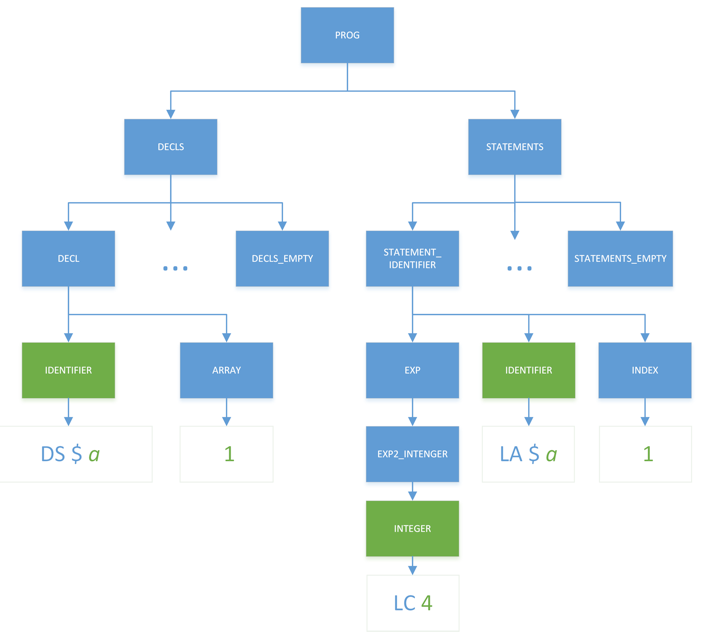
\includegraphics[width=1.0\linewidth]{Maschinencode.png}
    \caption{Maschinencode-Erzeugung durch CodeGenerator}\label{fig:codegenerator}
\end{figure}
